\documentclass[a4paper,12pt]{report} % размер бумаги устанавливаем А4, шрифт 12 пунктов
\usepackage[T2A]{fontenc} % поддержка кириллицы в ЛаТеХ
\usepackage[utf8]{inputenc} % настройка кодировки
\usepackage[english,russian]{babel} % Определение языков в документе
\usepackage{amssymb,amsfonts,amsmath,mathtext,cite,enumerate,float} % подключаем нужные пакеты расширений
\usepackage{indentfirst} % делать отступ в начале параграфа
\usepackage{tabularx} % продвинутые таблицы
% \usepackage{showkeys} % раскомментировать, чтобы в документе были видны ссылки на литературу, рисунки и таблицы
\usepackage[labelsep=period]{caption} % заменить умолчальное разделение ':' на '.' в подписях к рисункам и таблицам
\usepackage[onehalfspacing]{setspace} % "умное" расстояние между строк - установить 1.5 интервала от нормального
\usepackage[final]{graphicx} % разрешить включение PostScript-графики
\graphicspath{{img/}} % Относительный путь к каталогу с рисунками

\usepackage{textcomp}
\newcommand*{\No}{\textnumero}

\makeatletter
\bibliographystyle{unstr} % Стиль библиографических ссылок БибТеХа - нумеровать в порядке упоминания в тексте
\renewcommand{\@biblabel}[1]{#1.} % Заменяем библиографию с квадратных скобок на точку в списке литературы
\makeatother

\def\labelitemi{--} % установка префикса немаркированного списка

% Настройка геометрии
\usepackage{geometry}
\geometry{left=2cm}
\geometry{right=1.5cm}
\geometry{top=1cm}
\geometry{bottom=2cm}

% настройка листинга
\usepackage{color} %% это для отображения цвета в коде
\usepackage{xcolor}
\usepackage{listings} %% собственно, это и есть пакет listings

\usepackage{hyperref}
\usepackage{multirow}
\usepackage{enumitem}

\DeclareCaptionFont{white}{\color{white}} %% это сделает текст заголовка белым
%% код ниже нарисует серую рамочку вокруг заголовка кода.
\DeclareCaptionFormat{listing}{\colorbox{gray}{\parbox{\textwidth}{#1#2#3}}}
\captionsetup[lstlisting]{format=listing,labelfont=white,textfont=white}
\lstset{ %
language=C, % выбор языка для подсветки (здесь это С)
basicstyle=\small\sffamily, % размер и начертание шрифта для подсветки кода
numbers=left, % где поставить нумерацию строк (слева\справа)
%numberstyle=\tiny, % размер шрифта для номеров строк
stepnumber=1, % размер шага между двумя номерами строк
numbersep=5pt, % как далеко отстоят номера строк от подсвечиваемого кода
backgroundcolor=\color{white}, % цвет фона подсветки - используем \usepackage{color}
showspaces=false, % показывать или нет пробелы специальными отступами
showstringspaces=false, % показывать или нет пробелы в строках
showtabs=false, % показывать или нет табуляцию в строках
frame=single, % рисовать рамку вокруг кода
tabsize=2, % размер табуляции по умолчанию равен 2 пробелам
captionpos=t, % позиция заголовка вверху [t] или внизу [b]
breaklines=true, % автоматически переносить строки (да\нет)
breakatwhitespace=false, % переносить строки только если есть пробел
escapeinside={\%*}{*)} % если нужно добавить комментарии в коде
}

% Меняем везде перечисления на цифра.цифра
\renewcommand{\theenumi}{\arabic{enumi}}
\renewcommand{\labelenumi}{\arabic{enumi}}
\renewcommand{\theenumii}{\arabic{enumii}}
\renewcommand{\labelenumii}{\arabic{enumi}.\arabic{enumii}.}
\renewcommand{\theenumiii}{\arabic{enumiii}}
\renewcommand{\labelenumiii}{\arabic{enumi}.\arabic{enumii}.\arabic{enumiii}.}

\renewcommand{\thesection}{\arabic{section}.}
% \renewcommand{\thesubsection}{\arabic{section}.\arabic{subsection}.}
\renewcommand{\thesubsection}{\arabic{subsection}.}
% \renewcommand{\thesubsubsection}{\arabic{section}.\arabic{subsection}.\arabic{subsubsection}.}
\renewcommand{\thesubsubsection}{\arabic{subsection}.\arabic{subsubsection}.}

\newtheorem{theorem}{Theorem}
\usepackage{subcaption}

\begin{document}
\def\figurename{Figure} % префикс к рисунками
\def\tablename{Table}
\newpage
\begin{titlepage}

\begin{center}\large{
    FEDERAL STATE AUTONOMOUS EDUCATIONAL INSTITUTION \\
    OF HIGHER EDUCATION \\*
    ITMO UNIVERSITY \\*
}\end{center}

\vspace{12em}

\begin{center}\large{
    Report \\
    on the practical task No. 8 \\
    <<Practical analysis of advanced algorithms>>
}\end{center}

\vspace{8.5em}

\flushright{Performed by}
\flushright{Sultan Zhumabaev}
\flushright{J4133c}
\vspace{1.5em}
\flushright{Accepted by}
\flushright{Dr Petr Chunaev}

\vspace{\fill}

\begin{center}
    St. Petersburg \\
    2020
\end{center}

\end{titlepage}

% \tableofcontents
\newpage
\subsection{Goal}\label{subsec:goal}

Practical analysis of advanced algorithms

\subsection{Formulation of the problem}\label{subsec:formulation-of-the-problem}

\paragraph{I.}
Choose an algorithm (interesting to you and not considered in the course) from the above-mentioned book sections.

\paragraph{II.}
Choose an algorithm interesting to you and proposed at most 10 years ago in a research paper for solving a certain practical problem (including optimization algorithms, graph algorithms, etc.).

\paragraph{III.}
Analyse the chosen algorithms in terms of time and space complexity, design technique used, etc.
Implement the algorithms (or use the existing ones from the
research paper) and produce several experiments.
Your experiments should differ of those in the research paper.
Analyse the results.

\subsection{Brief theoretical part}\label{subsec:brief-theoretical-part}

\textit{Dynamic Programming} is a technique in computer programming that helps to efficiently solve a class of problems that have overlapping subproblems and optimal substructure property.
Such problems involve repeatedly calculating the value of the same subproblems to find the optimum solution.

\textit{A divide and conquer algorithm} is a strategy of solving a large problem by
\begin{itemize}
    \item breaking the problem into smaller sub-problems;
    \item solving the sub-problems;
    \item combining them to get the desired output.
\end{itemize}

\textit{Floyd-Warshall Algorithm} is an algorithm for finding the shortest path between all the pairs of vertices in a weighted graph [1].
This algorithm works for both the directed and undirected weighted graphs.
But, it does not work for the graphs with negative cycles (where the sum of the edges in a cycle is negative).

This algorithm follows the dynamic programming approach to find the shortest paths.

\textit{Algorithm for finding an intersection line of two objects} was proposed in 2019 [2].
Proposed method consists of following steps: first of all, it states the fact of intersection of two objects.
Objects are transferred to two-dimensional space.
Then, it searches for intersection lines of polygons from which objects consist.
A set of segments is obtained.
Finally, it builds line $L$ and plane $P$ and searches for the point of intersection (Figure~\ref{ris:soliddemo}).

This algorithm follows the divide and conquer approach to check the fact of intersection.

\begin{figure}[H]
    \center
    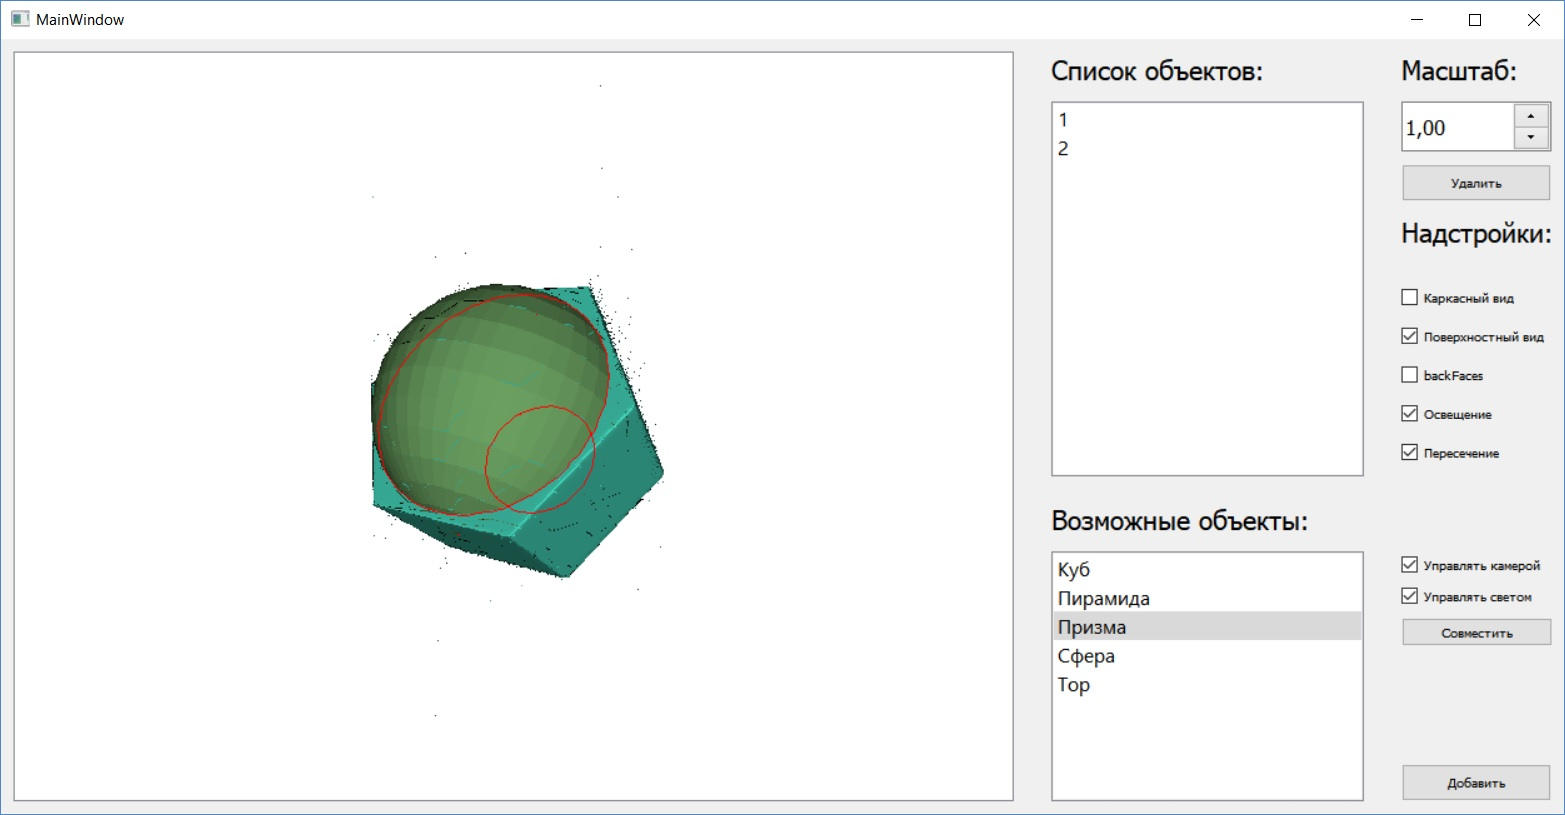
\includegraphics[width=\textwidth]{img/soliddemo.jpg}
    \caption{Intersection of a sphere and a prism}
    \label{ris:soliddemo}
\end{figure}

\subsection{Results}\label{subsec:results}

As a result of measuring the \textit{Floyd-Washall} algorithm for the matrix $\lvert V \rvert = 100$ and $\lvert E \rvert = 500$, the following result is obtained: \textit{1.325 ms}.

\textit{Time Complexity} - there are three loops.
Each loop has constant complexities.
So, the time complexity of the \textit{Floyd-Warshall} algorithm is $O(n^3)$.

\textit{Space Complexity} of the \textit{Floyd-Warshall} algorithm is $O(n^2)$.

\textit{Floyd-Warshall} algorithm applications:
\begin{itemize}
    \item to find the shortest path is a directed graph;
    \item to find the transitive closure of directed graphs;
    \item to find the Inversion of real matrices;
    \item for testing whether an undirected graph is bipartite.
\end{itemize}

For the \textit{intersection line search algorithm} (ILSA), we analyze the optimal number of threads for solving the problem (16 logical cores on the tested machine):

\begin{figure}[H]
    \center
    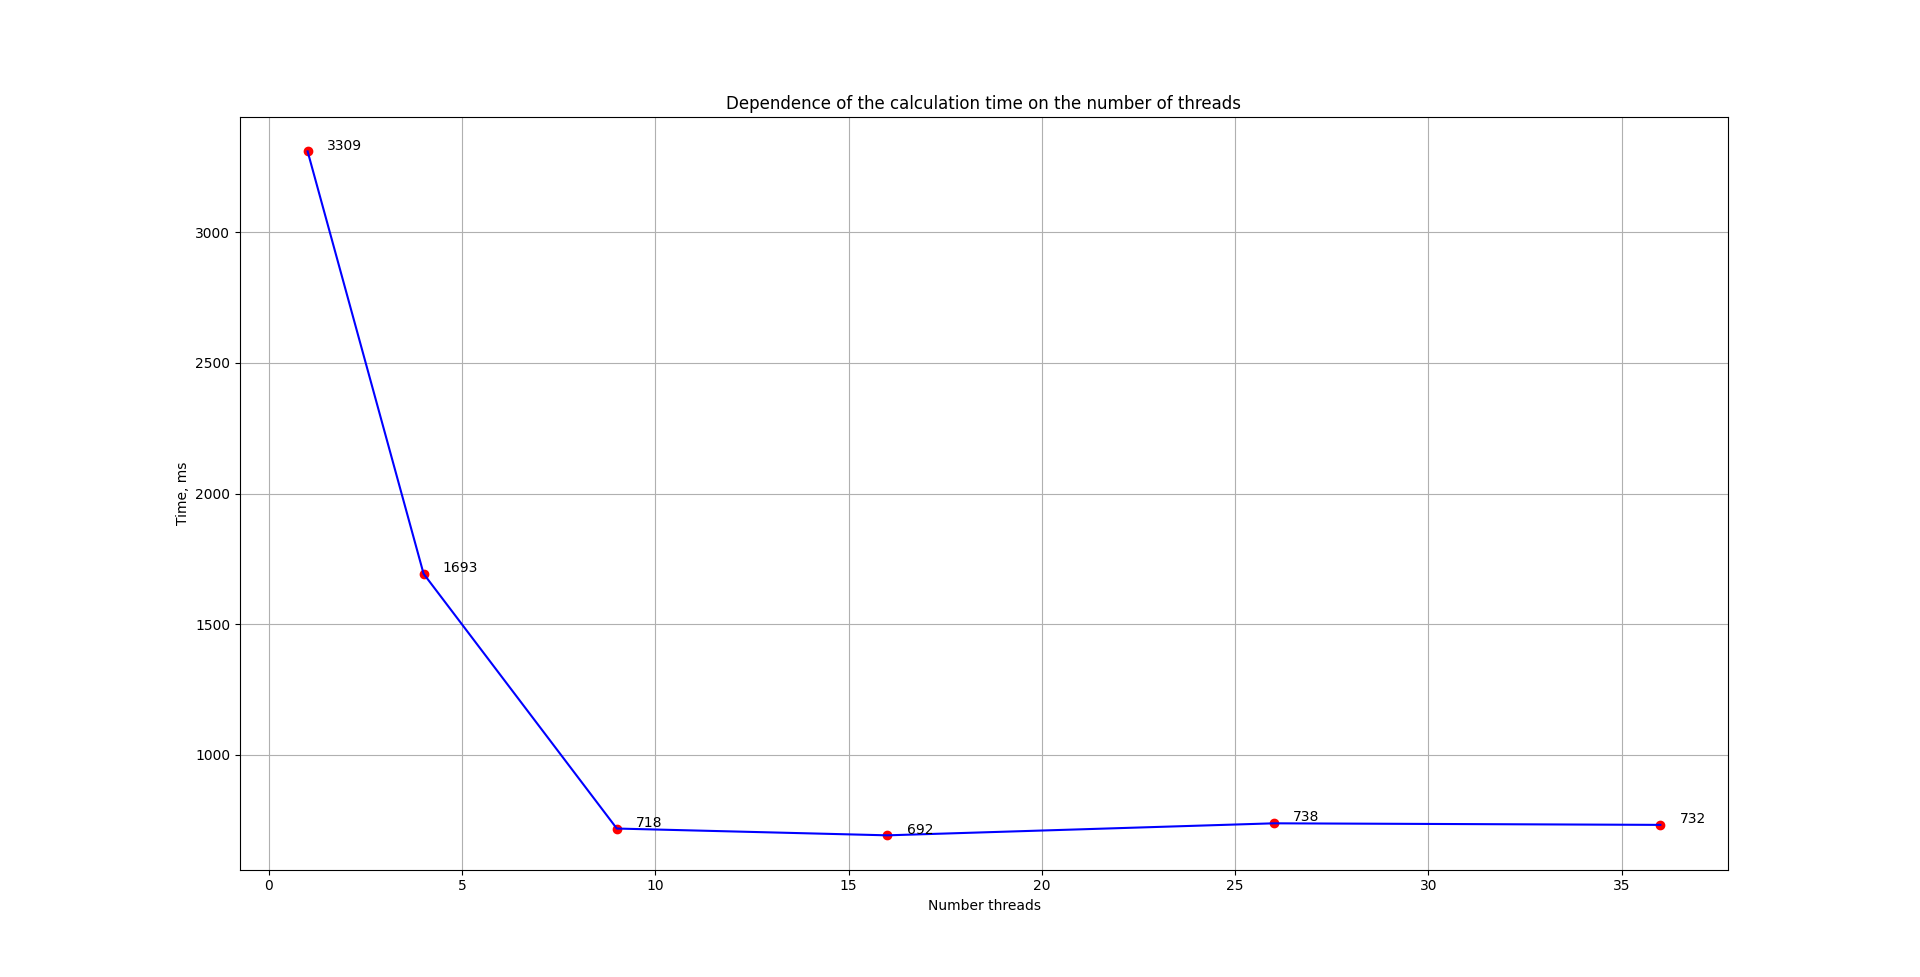
\includegraphics[width=\textwidth]{img/plot.png}
    \caption{Time complexity of ILSA}
    \label{ris:plot}
\end{figure}

A sphere (\textit{3816 polygons}) and a prism (\textit{1426 polygons}) were used for the experiment (Figure~\ref{ris:plot}).

As the number of threads increases, the speed of the algorithms increases.
Since there are only 16 logical cores in the system, increasing the number of threads from 25 to 36 does not give a noticeable gain in time.
In contrast, the calculation time increases as quasi-parallel calculations begin.
As a result, the use of parallel computing allowed to increase the speed of work by 4.78 times.

\textit{Time Complexity} - there are two loops.
Each loop has constant complexities.
So, the time complexity of the \textit{ILSA} algorithm is $O(NM)$, where $N, M$ are the numbers of polygons of the first and second object, respectively.

\textit{Space Complexity} of the \textit{ILSA} algorithm is $O(NM)$.

\subsection{Conclusion}\label{subsec:conclusion}

This paper is analyzed two advanced algorithms.

\subsection{References}\label{subsec:references}
\begin{enumerate}[label={[\arabic*]}]
    \item Cormen T.H., Leiserson C.E., Rivest R.L, Stein C. Introduction to Algorithms.\ Third Edition.\ The MIT Press, 2009.
    \item Жумабаев С.К., Шикуть А.В. Линия пересечения двух объектов // Новые информационные технологии в автоматизированных системах.\ 2019.\ №22.\ URL: https://cyberleninka.ru/article/n/liniya-peresecheniya-dvuh-obektov (дата обращения: 31.10.2020).
\end{enumerate}

\subsection{Appendix}\label{subsec:appendix}

The source code is located \href{https://github.com/vanSultan/anal_dev_algo/tree/develop/lab_08}{here}: \url{https://github.com/vanSultan/anal_dev_algo/tree/develop/lab_08}.

\end{document}
